\documentclass{article}
\usepackage{minted}
\usepackage{graphicx}
\usepackage{caption}
\author{Monnier Killian\and André Émilien \and Ikrame Bakkari}
\title{Project 2: Explainable Artificial Intelligence and Cybersecurity}
\begin{document}
\maketitle
\section{Introduction}
Neural networks with fine-tuned weights outperform ML algorithms but their results are difficult to interpret, and, one cannot manually define a rule in the prediction process.\par
This lack of interpretability prevents banks and other financial institutions from using them.\par
Explainable AI is a field of study that aims to address these issues.\par
Another advantage of XAI is when rules are defined it makes it impossible for training biases.\par
If an Intrusion Detection System (IDS) use XAI in Security Information and Event Management (SIEM). A SIEM analyst will have explainations on detected threats to take important decisions such as shutting down the Information System (IS).\par
The use case we are dealing with in this project is the detection of breast cancers. Sensitivity ranges between 53.1 and 73\% among radiologists and specificity is 96\%. [2][3]
\section{State of the Art}
Current explainable IA methods are SHAP and BRCG. Protodash shows samples from training dataset which are similar to given sample, it shows similarities and differences between them, etc. For end user LIME, SHAP and CEM explain which features in the input instance are contributing in model's final decision and how model's decision can be changed by tweaking their values. [1]
\section{XAI on a breast cancer classifier}
We use a LogisticRegression classifier on the Wisconsin dataset composed of 569 elements of 30 features
\begin{minted}[frame=lines]{python}
# Load breast cancer
from sklearn.datasets import load_breast_cancer
data = load_breast_cancer()

# Display the shape of the data
print(data.data.shape)

# Display the column names
print(data.feature_names)

# Charger le dataset
X, y = load_breast_cancer(return_X_y=True)
\end{minted}
\begin{verbatim}
(569, 30)
['mean radius' 'mean texture' 'mean perimeter' 'mean area'
 'mean smoothness' 'mean compactness' 'mean concavity'
 'mean concave points' 'mean symmetry' 'mean fractal dimension'
 'radius error' 'texture error' 'perimeter error' 'area error'
 'smoothness error' 'compactness error' 'concavity error'
 'concave points error' 'symmetry error' 'fractal dimension error'
 'worst radius' 'worst texture' 'worst perimeter' 'worst area'
 'worst smoothness' 'worst compactness' 'worst concavity'
 'worst concave points' 'worst symmetry' 'worst fractal dimension']
\end{verbatim}
The train-test split is 0.2, we used a scikit StandardScaler to scale the data and our model is a logistic regression.
\begin{minted}[frame=lines]{python}
# Train test split
from sklearn.model_selection import train_test_split
# Séparer les données en ensemble d'entraînement et de test
X_train, X_test, y_train, y_test = train_test_split(X, y, test_size=0.2, random_state=42)   

# Scale the data
from sklearn.preprocessing import StandardScaler
scaler = StandardScaler()
X_train = scaler.fit_transform(X_train)
X_test = scaler.transform(X_test)

# Train the model
from sklearn.linear_model import LogisticRegression
model = LogisticRegression()
model.fit(X_train, y_train)
\end{minted}
We got a sensitivity of 96\% and a specificity of 99\%, thus beating radiologist's results. However, our dataset maybe to small to get a good overlook of our model performance.\par
Thanks to SHAP we have an overview of the attributes contributions overall and the attributes contributions for one prediction.
\begin{center}
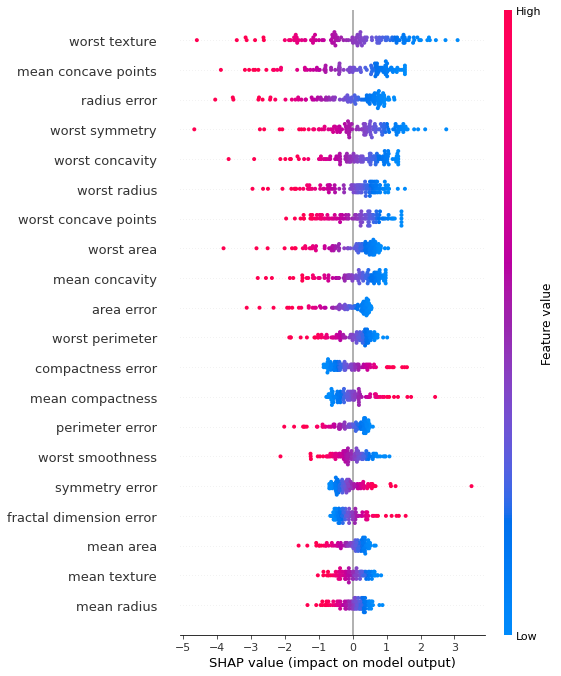
\includegraphics[width=10cm]{kiki-shap-summary-plot.png}
	\captionof{figure}{Attributes contributions overall}
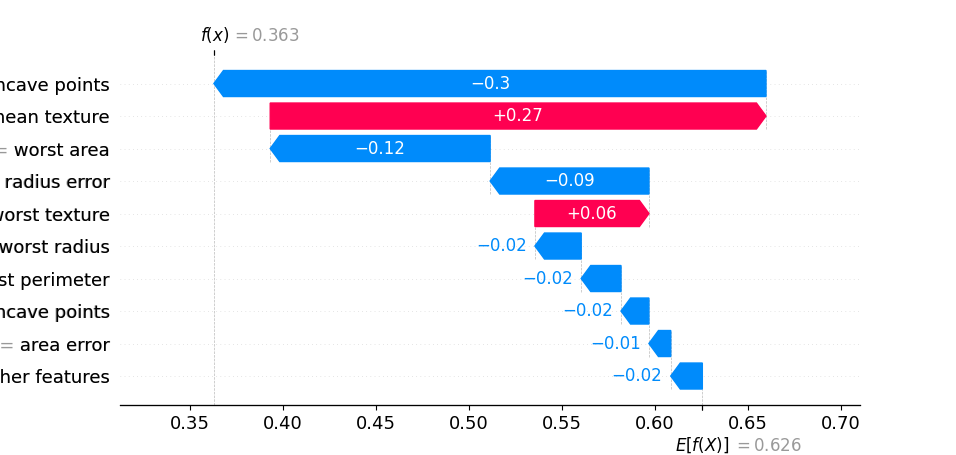
\includegraphics[width=10cm]{waterfall.png}
	\captionof{figure}{Attributes contributions in one prediction}
\end{center}
\section{Conclusion}
From our project perspective, results are promising but the model should be evaluated on a greater dataset before making any assumptions of its potential application in real use case.\par
From a global perspective, XAI is promising and have the potential to be deployed in the medical and banking sectors, where its ability to explain deep neural networks, which already have greater performances over human predictions, will allow them to be deployed.
\section{References}
[1] : Mane, Shraddha \& Rao, Dattaraj. (2021). Explaining Network Intrusion
Detection System Using Explainable AI Framework.\newline
[2] : Britton P, Warwick J, Wallis MG, O'Keeffe S, Taylor K, Sinnatamby R, Barter S, Gaskarth M, Duffy SW, Wishart GC. Measuring the accuracy of diagnostic imaging in symptomatic breast patients: team and individual performance. Br J Radiol. 2012 Apr;85(1012):415-22. doi: 10.1259/bjr/32906819. Epub 2011 Jan 11. PMID: 21224304; PMCID: PMC3486650.\newline
[3] : Mattie Salim , Karin Dembrower, Martin Eklund, Peter Lindholm, Fredrik Strand. Range of Radiologist Performance in a Population-based Screening Cohort of 1 Million Digital Mammography Examinations.
\end{document}
